\documentclass[10pt,a4j,twoside]{jarticle}
\usepackage{amsmath}
%\usepackage{mathabx}
%\usepackage{psfig}
\usepackage{graphicx} % use \includegrahpics
%\usepackage{Tabular}

\usepackage{enumsty}

\def\figref#1{図~\ref{#1}}
\def\tabref#1{表~\ref{#1}}
\def\eqref#1{(\ref{#1})~式}
\def\eqrefbare#1{\ref{#1}}
\def\secref#1{\ref{#1}~節}
\def\Theoref#1{定理~\ref{#1}}
\def\Lemref#1{補題~\ref{#1}}

\pagestyle{bothstyle}
\makeatletter
%\def\@oddfoot{\hbox to \textwidth{\fhil \thepage \hfil}}
%\def\@oddfoot{\reset@font\hfil\thepage\hfil}%
\makeatother

\makeatletter
\@addtoreset{equation}{section}
\renewcommand{\theequation}{\thesection.\@arabic\c@equation}
\makeatother

%\usepackage{showlabel}

%%----------------------------------------------------------------------
%%
\usepackage{bm}
%\def\V#1{\mbox{\boldmath $#1$}}
%\def\M#1{\mbox{\boldmath $#1$}}
%\def\S#1{\mbox{\boldmath $#1$}}
%\def\Ts#1{\mbox{\boldmath $#1$}}
\def\V#1{{\bm{#1}}}
\def\M#1{{\bm{#1} }}
\def\S#1{{\bm{#1}}}
\def\Ts#1{{\bm{#1}}}

\usepackage{amsmath}
\usepackage{amssymb}
\usepackage{amsfonts}

\def\SetNat{\mathbb{N}}  % 自然数集合
\def\SetInt{\mathbb{Z}}  % 整数集合
\def\SetRat{\mathbb{Q}}  % 有理数集合
\def\SetReal{\mathbb{R}} % 実数集合
\def\SetComp{\mathbb{C}} % 複素数集合

\def\Deg#1{^{\left< #1 \right>}}  % 次数
\def\Cxc#1{{#1}^{\dagger}} % 複素共役

\def\Abs#1{\left| #1 \right|}

\def\MtxK#1#2{\left[ \begin{array}[c]{#1} #2 \end{array} \right]}
\def\Vec#1{\MtxK{c}{#1}}
\def\Mtxxxx#1{\MtxK{cccc}{#1}}
\def\Mtxx#1{\MtxK{cc}{#1}}
\def\Mtx#1{\MtxK{c}{#1}}
\def\Tsr#1{\MtxK{c}{#1}}

\def\Dpd{\times} %% 直積記号 : direct product
\def\Kpd{\otimes} %% クロネッカー積記号 : Kronecker product
\def\DpA#1{\bar{#1}}  %% 直積の値の頭につけるアクセント

\def\MxA#1{\hat{#1}}  %%  混合分布につけるアクセント

\def\Est#1{\hat{#1}}    %% estimate
\def\Apx#1{\tilde{#1}}  %% approx

\def\Av#1{\left|#1\right|}
\def\SD#1{\sigma_{#1}}
\def\Var#1{\SD{#1}^2}
\def\Avg#1{\mu_{#1}}
\def\Xpt#1{\bar{#1}}  %% 期待値

\def\Seq#1{\left\{ #1 \right\}}
\def\Set#1{\left\{ #1 \right\}}
\def\Tuple#1{\left< #1 \right>}

\makeatletter
  \def\@LkS{{\cal L}}    %% likelihood Symbol
  \def\@LkF[#1]{\@LkS\left(#1\right)}    %% likelihood func.
  \def\Lk{\@ifnextchar[{\@LkF}{\@LkS}% ]
         }
\makeatother

\makeatletter
  \def\@PrSym{{\cal P}}
  \def\Pr{\@ifnextchar[{\@Pr}{\@PrSym}% ]
  }
  \def\@Pr[#1]{\@PrSym\left(#1\right)}

  %% Gaussian  G[x;\mu,\sigma]
  \def\@GSym{{\cal G}}        
  \def\G{\@ifnextchar[{\@G}{\@GSym}% ]
  }
  \def\@G[#1]{\@GSym\left(#1\right)}

%% 二項分布・Binomial 
  \def\@BnSym{{\cal B}}
  \def\Bn{\@ifnextchar[{\@Bn}{\@BnSym}% ]
  }
  \def\@Bn[#1]{\@BnSym\left(#1\right)}

%% 幾何分布・geometric distribution
  \def\@GmSym{\mathsf{g}}
  \def\Gm{\@ifnextchar[{\@Gm}{\@GmSym}% ]
  }
  \def\@Gm[#1]{\@GmSym\left(#1\right)}

%% noise
  \def\nz{\epsilon}	


\makeatother


\def\EqDesc#1{\mbox{\ \ \ ; #1}}


\makeatletter
\def\Lp{\@ifnextchar[{\@Lp}{{\cal L}}} %% ラプラス変換 \Lp[f] or \Lp(f)
\def\@Lp[#1]{\Lp{}\left[#1\right]}
\def\ILp{\@ifnextchar[{\@ILp}{{\cal L}^{-1}}} %% ラプラス変換 \Lp[f] or \Lp(f)
\def\@ILp[#1]{\ILp{}\left[#1\right]}
\makeatother

\def\Conv{\ast}  %% 畳み込み積分 (Convolution Integral)
\def\Comb#1#2{{}_{#1}C_{#2}}

%%======================================================================

\def\Where{\mbox{\hspace{3em}} ; \mbox{\hspace{1em}}}
\def\where0pt{\makebox[0pt][l]{\mbox{where}} \nonumber}


\def\MyBox#1{{\unitlength=#1 \framebox(1,1){}}}
\def\MyFillBox#1{\rule{#1}{#1}}
\def\EOTH{\hfill\MyBox{.5em}}
\def\QED{\hfill\MyFillBox{.5em}}

\newenvironment{Note}[1]{%
%  \paragraph*{ノート: #1} \fill \rule{0.5\textwidth}{1pt}
  \paragraph{\protect\MyFillBox{1em} ノート--- #1} \hrule%
  \hfill 
}{%
  \hfill\MyBox{1em}\hrule
  \ \\
}

%%======================================================================

\newif\ifWideBoxedEqnarray
\WideBoxedEqnarraytrue
\WideBoxedEqnarrayfalse

\newenvironment{BoxedEqnarray}{%
  \vspace{-4ex}
  \begin{center}%
    \begin{tabular}[c]{|c|} \hline%
      \begin{minipage}[c]{\textwidth}  %{width}
      \ifWideBoxedEqnarray%
        \vspace{-0.5ex} %
      \else%
        \vspace{-2.3ex} %
      \fi%
        \begin{eqnarray}%
}{%
        \end{eqnarray}%
      \end{minipage}%
      \ifWideBoxedEqnarray%
        \\%
      \else%
        % nothing
      \fi%
%      \\
      \\ \hline%
    \end{tabular}
  \end{center}%
}

%%======================================================================

\def\DefPrefix{定義}
\def\LemmaPrefix{補題}
\def\TheoremPrefix{定理}
\newtheorem{genericTheorems}{GenericTheorem}[section]
\newtheorem{xDef}[genericTheorems]{\DefPrefix}
\newtheorem{xLemma}[genericTheorems]{\LemmaPrefix}
\newtheorem{xTheorem}[genericTheorems]{\TheoremPrefix}

\newenvironment{Lemma}{%
  \begin{xLemma}%
    \addcontentsline{toc}{subparagraph}{%
      \fbox{\LemmaPrefix \thexLemma}}
  \ \\
}{%
  \EOTH%
  \end{xLemma}%
}

\newenvironment{Theorem}{%
  \begin{xTheorem}%
    \addcontentsline{toc}{subparagraph}{%
      \fbox{\TheoremPrefix \thexLemma}}
  \ \\
}{%
  \EOTH
  \end{xTheorem}%
}


\newenvironment{Proof}{%
  \subsubparagraph*{証明}\par%
}{%
  \QED%
}





%\iftrue
\iffalse
\includeonly{
%  S010/secBody.primePair,
%  S020/secBody.factorial,
%  S030/secBody.changeShort,
%  S040/secBody.complexNum,
  S050/secBody.threeObj
  }
\fi

%\def\ClearPage{\clearpage}
\def\ClearPage{\cleardoublepage}

\begin{document}
%%----------------------------------------------------------------------
\title{IS Lab. 問題集}
\author{野田五十樹}
\date{%
  {\scriptsize
  \begin{tabular}[c]{|l|l|} \hline
  2024/02/23 & 素数組問題 \\ \hline
  2024/02/23 & 階乗問題 \\ \hline
  2024/02/23 & お釣り問題 \\ \hline
  2024/02/23 & 複素数問題 \\ \hline
  2024/08/15 & 三体宇宙船問題 \\ \hline
 \end{tabular}
  }
}
\maketitle
%%----------------------------------------------------------------------

\setcounter{tocdepth}{10}

\iftrue
%\iffalse
\ClearPage
\tableofcontents
\ClearPage\cleardoublepage
\fi

%%----------------------------------------------------------------------
\section{素数の組}
\label{s:素数の組}
%% - - - - - - - - - - - - - - - - - - - - - - - - - - - - - - - - - - -

%%--------------------------------------------------
\subsection{問題}
\label{ssec:素数の組:問題}
%% - - - - - - - - - - - - - - - - - - - - - - - - -

$p^q + q^p$ が素数になる素数の組 $\Tuple{p,q}$ を全て求めよ。
ただし、$p<q$ とする。

\clearpage
%%--------------------------------------------------
\subsection{解答}
\label{ssec:素数の組:解答}
%% - - - - - - - - - - - - - - - - - - - - - - - - -

$p,q$ が共に奇数の素数とする。
その場合、$p^q, q^p$ は共に2より大きい奇数となる。
よって、$p^q + q^p$ は2より大きい偶数になり、素数ではない。

よって、$p,q$ はいずれかは偶数の素数、すなわち $2$ となる。
また、$p < q$ から、$p = 2$ となる。

$q = 3$ の場合、$p^q + q^p = 2^3 + 3^2 = 8 + 9 = 17$ となり、素数である。
よって、 $\Tuple{2,3}$ は条件を満たす組となる。

$q > 3$ の場合、
2の倍数、3の倍数は素数ではないので、
$q = 6k \pm 1$ と表される。
よって、
  %%$$$$$$$$$$$$$$$$$$$$$$$$$$$$$$$$$$$$$$$$$$$$$$$$$$$$$$$$$$$$$$$$$$$$$$
  \begin{eqnarray}
    p^q + q^p
      & = &
        2^{6 k \pm 1} + (6 k \pm 1)^2
  \\
      & = &
        2 + 1   \mod 3
  \\
      & = &
        3
  \\
      & = &
        0   \mod 3
  \end{eqnarray}
  %%$$$$$$$$$$$$$$$$$$$$$$$$$$$$$$$$$$$$$$$$$$$$$$$$$$$$$$$$$$$$$$$$$$$$$$
となり、かならず 3 で割り切れる。
すなわち、素数ではない。

よって、$q > 3$ の場合、条件を満たす組 $\Tuple{p,q}$ は存在しない。

よって、条件を満たす素数の組は、$\Tuple{2,3}$ のみである。
\QED






\ClearPage\cleardoublepage
%%----------------------------------------------------------------------
\section{階乗に関する問題}
\label{s:階乗}
%% - - - - - - - - - - - - - - - - - - - - - - - - - - - - - - - - - - -

%%--------------------------------------------------
\subsection{階乗を割った余り}
\label{ssec:階乗:階乗を割った余り}
%% - - - - - - - - - - - - - - - - - - - - - - - - -
%%-----------------------------
\subsubsection{問題}
\label{sssec:階乗:階乗を割った余り:問題}
%% - - - - - - - - - - - - - -

$100 !$ を $97$ で割った余りはいくらか?


\clearpage
%%------------------------------
\subsubsection{解答}
\label{sssec:階乗:階乗を割った余り:解答}
%% - - - - - - - - - - - - - - -

$100 ! = 100 \cdot 99 \cdot 98 \cdot 97 \cdot 96 \ldots$ であるので、
$100!$ は $97$ を因子として持つ。
よって、$100!$ を $97$ で割った余りは 0 である。


%%------------------------------
\subsubsection{参考: Wilson の定理}
\label{sssec:階乗:階乗を割った余り:参考}
%% - - - - - - - - - - - - - - -

\begin{Theorem}
  $p$ が素数ならば、 $(p-1)! = -1 \mod p$ である。
  \\
  逆に、自然数 $p > 1$ に対し $(p-1)! = -1 \mod p$ ならば、
  $p$ は素数である。
\end{Theorem}
  

\clearpage
%%--------------------------------------------------
\subsection{階乗の階乗を割った余り}
\label{ssec:階乗:階乗の階乗を割った余り}
%% - - - - - - - - - - - - - - - - - - - - - - - - -

%%-----------------------------
\subsubsection{問題}
\label{sssec:階乗:階乗の階乗を割った余り:問題}
%% - - - - - - - - - - - - - -

$(100 !)!$ を $(99!)^{100}$ で割った余りはいくらか?


\clearpage
%%------------------------------
\subsubsection{解答}
\label{sssec:階乗:階乗の階乗を割った余り:解答}
%% - - - - - - - - - - - - - - -

\begin{Lemma}
  自然数$n,m$ で、$n \ge m$ の時、
  $n!$ は $m! \cdot (n-m)!$ で割り切れる。
\end{Lemma}

\begin{Theorem}
  自然数の列 $\Seq{k_1, k_2, \cdots, k_n}$ を考える、この時、
  $\left( \sum_{i=1}^{n} k_i \right) !$ は
  $\prod_{i=1}^{n} k_i !$ で割り切れる。
\end{Theorem}

$k_1 = k_2 = \cdots = k_{100!} = 99!$ とすれば、
$\sum_{i=1}^{100} k_i = 100 \cdot 99! = 100!$ であり、
$\prod_{i=1}^{100} k_i = (99!)^{100} $ である。
これにより、上記の定理を使うと、
$(100!)!$ は $(99!)^{100}$ で割り切れる。
\QED





\ClearPage\cleardoublepage
%%----------------------------------------------------------------------
\section{お釣りが足りている}
\label{s:お釣り}
%% - - - - - - - - - - - - - - - - - - - - - - - - - - - - - - - - - - -

%%--------------------------------------------------
\subsection{問題}
\label{ssec:お釣り:問題}
%% - - - - - - - - - - - - - - - - - - - - - - - - -

%%--------------------------------------------------
\subsubsection{具体問題}
\label{sssec:お釣り:問題:具体問題}
%% - - - - - - - - - - - - - - - - - - - - - - - - -

ある商人が1個50円のおもちゃを10個売っているとする。
お客は、各々1つずつそのおもちゃを買うとし、
支払いには、100円玉か50円玉でしか支払わないとする。
商人は、最初、お釣り用の50円玉を4枚用意しているとする。
おもちゃ10個が売り切れた時、
商人の手元には50円玉が2枚あった。

この場合、お客が支払った50円玉・100円玉の順序の場合の数は何通りあるか?

%%--------------------------------------------------
\subsubsection{一般化問題}
\label{sssec:お釣り:問題:一般化問題}
%% - - - - - - - - - - - - - - - - - - - - - - - - -

上記の問題で、おもちゃの数を $n$ 個、
最初に用意した50円玉の枚数を $m$ 枚、
最後の残った50円玉の枚数を $l$ 枚とした時、
お客が支払った50円玉・100円玉の順序の場合の数は何通りあるか?


\clearpage
%%--------------------------------------------------
\subsection{解答}
\label{ssec:お釣り:解答}
%% - - - - - - - - - - - - - - - - - - - - - - - - -

%%--------------------------------------------------
\subsubsection{具体問題}
\label{sssec:お釣り:解答:具体問題}
%% - - - - - - - - - - - - - - - - - - - - - - - - -

問題の設定により、
おもちゃが1つ売れる毎に50円玉は1枚増えるか1枚減るかたちで
枚数が変化する。

その様子を表したのが、\figref{fig:S030/Figs/Figure.change.p01}である。
横軸は売れたおもちゃの数、
縦軸が50円玉の数であり、
$(0,4)$ から出発して、$(10,2)$ に至る斜めの碁盤目の経路を辿ることになる。

この内、お釣りの50円玉が足らなくなるのは、図の赤い経路を通る場合である。
つまり、\figref{fig:S030/Figs/Figure.change.p01}で示される碁盤目のうち、
赤い経路を通らない経路の数を数えれば良い。

まず、赤い経路を無視して、全ての碁盤目の経路を数え上げると、
10個の選択肢の中から順不同で4つ選ぶ場合の数であるので、
  %%$$$$$$$$$$$$$$$$$$$$$$$$$$$$$$$$$$$$$$$$$$$$$$$$$$$$$$$$$$$$$$$$$$$$$$
  \begin{eqnarray}
    N_{\text{all}} & = & _{10}C_{4}
  \\
      & = &
        \frac{10!}{4! 6!}
  \\
      & = &
        210
  \end{eqnarray}
  %%$$$$$$$$$$$$$$$$$$$$$$$$$$$$$$$$$$$$$$$$$$$$$$$$$$$$$$$$$$$$$$$$$$$$$$
  
次に、
全て数え上げた中から、お釣りが足らなかった経路を取り上げる。
この時、お釣りが足らなくなった瞬間から、
50円玉の残り数を示す碁盤目を辿る方向を反転させるとする。
すると、
その経路が行き着く先は、
\figref{fig:S030/Figs/Figure.change.p02}のように、
$y=-1$ のところで鏡像にした経路を描く。
よって、その後、$(10,2)$ にたどり着いていた経路は、
この鏡像にした経路の中では、$(10,-4)$ に辿り着く。

そこで、$(0,4)$から$(10,-4)$ に辿る経路を数え上げると、
10個の選択肢の中から1つ順不同で選び出す場合の数であるので、
  %%$$$$$$$$$$$$$$$$$$$$$$$$$$$$$$$$$$$$$$$$$$$$$$$$$$$$$$$$$$$$$$$$$$$$$$
  \begin{eqnarray}
    N_{\text{short}} & = & _{10}C_{1}
  \\
      & = &
        \frac{10!}{1! 9!}
  \\
      & = &
        10
  \end{eqnarray}
  %%$$$$$$$$$$$$$$$$$$$$$$$$$$$$$$$$$$$$$$$$$$$$$$$$$$$$$$$$$$$$$$$$$$$$$$

  %%$$$$$$$$$$$$$$$$$$$$$$$$$$$$$$$$$$$$$$$$$$$$$$$$$$$$$$$$$$$$$$$$$$$$$$
  \begin{eqnarray}
    N_{\text{ans}} & = & N_{\text{all}} - N_{\text{short}}
  \\
      & = & 210 - 10
  \\
      & = & 200
  \end{eqnarray}
  %%$$$$$$$$$$$$$$$$$$$$$$$$$$$$$$$$$$$$$$$$$$$$$$$$$$$$$$$$$$$$$$$$$$$$$$

よって答えは、200通り。


%%FFFFFFFFFFFFFFFFFFFFFFFFFFFFFFFFFFFFFFFFFFFFFFFFFFFFFFFFFFFFFFFFFFFFFF
\begin{figure}
  \begin{minipage}[c]{.49\linewidth}  %{width}
  \centering
  \includegraphics[width=5cm]{S030/Figs/Figure.change.p01.eps}
  \caption{お釣り玉の残数の変化経路図}
  \label{fig:S030/Figs/Figure.change.p01}
  \end{minipage}~
%\end{figure}
%%FFFFFFFFFFFFFFFFFFFFFFFFFFFFFFFFFFFFFFFFFFFFFFFFFFFFFFFFFFFFFFFFFFFFFF
%%FFFFFFFFFFFFFFFFFFFFFFFFFFFFFFFFFFFFFFFFFFFFFFFFFFFFFFFFFFFFFFFFFFFFFF
%\begin{figure}[b]
  \begin{minipage}[c]{.49\linewidth}  %{width}
  \centering
  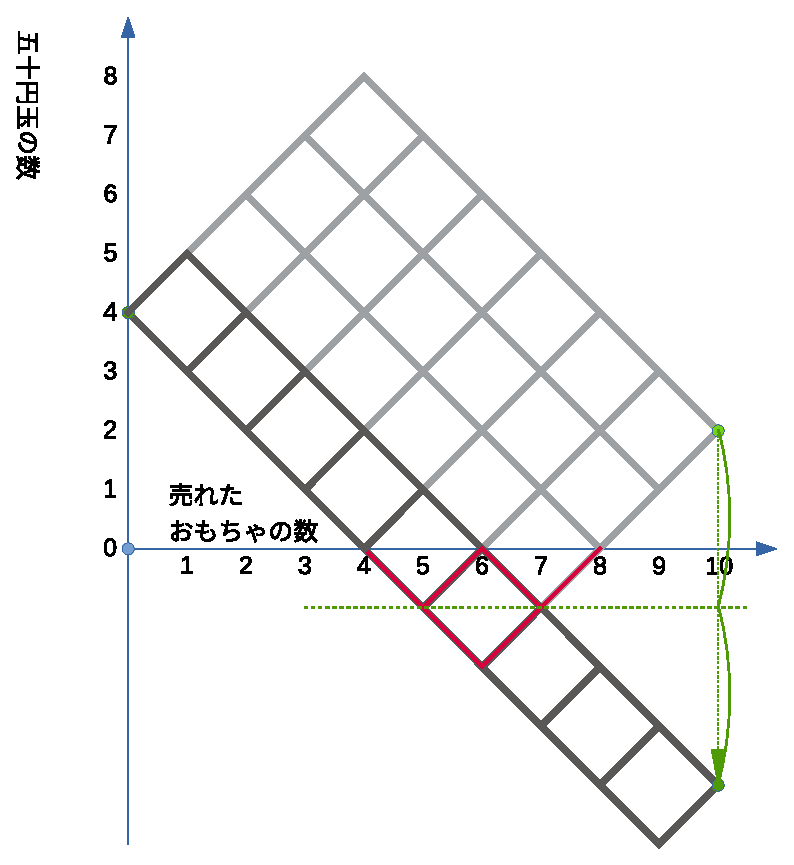
\includegraphics[width=5cm]{S030/Figs/Figure.change.p02.eps}
  \caption{お釣り玉が足らなくなる場合の残数の変化経路図}
  \label{fig:S030/Figs/Figure.change.p02}
  \end{minipage}
\end{figure}
%%FFFFFFFFFFFFFFFFFFFFFFFFFFFFFFFFFFFFFFFFFFFFFFFFFFFFFFFFFFFFFFFFFFFFFF


%%--------------------------------------------------
\subsubsection{一般化問題}
\label{sssec:お釣り:解答:一般化問題}
%% - - - - - - - - - - - - - - - - - - - - - - - - -

上記と同じ考え方をすると、
お釣りが足らなくなる場合の考えずに全ての経路を考えると、
$(0,m)$ から $(n,l)$ に至る斜めの碁盤目の経路となる。
この経路の数は
$n$ の候補の中から $\frac{n - (m-l)}{2}$ を順不同で選び出す場合の数であるので、
以下のように表せる。
  %%$$$$$$$$$$$$$$$$$$$$$$$$$$$$$$$$$$$$$$$$$$$$$$$$$$$$$$$$$$$$$$$$$$$$$$
  \begin{eqnarray}
    N_{\text{all}} & = & _{n}C_{\frac{n - (m-l)}{2}}
  \end{eqnarray}
  %%$$$$$$$$$$$$$$$$$$$$$$$$$$$$$$$$$$$$$$$$$$$$$$$$$$$$$$$$$$$$$$$$$$$$$$

一方、お釣りが足りなくなる経路の数は、
$(0,m)$ から $(n,-l-2)$ に至る斜めの碁盤目の経路となる。
この経路の数は
$n$ の候補の中から $\frac{n - (m+l+2)}{2}$ を順不同で選び出す場合の数であるので、
以下のように表せる。
  %%$$$$$$$$$$$$$$$$$$$$$$$$$$$$$$$$$$$$$$$$$$$$$$$$$$$$$$$$$$$$$$$$$$$$$$
  \begin{eqnarray}
    N_{\text{short}} & = & _{n}C_{\frac{n - (m+l+2)}{2}}
  \end{eqnarray}
  %%$$$$$$$$$$$$$$$$$$$$$$$$$$$$$$$$$$$$$$$$$$$$$$$$$$$$$$$$$$$$$$$$$$$$$$

よって、お釣りが足らなくならない経路の数は、
以下のように表すことができる。
  %%$$$$$$$$$$$$$$$$$$$$$$$$$$$$$$$$$$$$$$$$$$$$$$$$$$$$$$$$$$$$$$$$$$$$$$
  \begin{eqnarray}
    N_{\text{ans}} & = & N_{\text{all}} - N_{\text{short}}
  \\
      & = & _{n}C_{\frac{n - (m-l)}{2}} - _{n}C_{\frac{n - (m+l+2)}{2}}
  \end{eqnarray}
  %%$$$$$$$$$$$$$$$$$$$$$$$$$$$$$$$$$$$$$$$$$$$$$$$$$$$$$$$$$$$$$$$$$$$$$$


\ClearPage\cleardoublepage
%%----------------------------------------------------------------------
\section{複素数に関する問題}
\label{s:複素数}
%% - - - - - - - - - - - - - - - - - - - - - - - - - - - - - - - - - - -

%%--------------------------------------------------
\subsection{1の$x$乗}
\label{ssec:複素数:1のx乗}
%% - - - - - - - - - - - - - - - - - - - - - - - - -
%%-----------------------------
\subsubsection{問題}
\label{sssec:複素数:1のx乗:問題}
%% - - - - - - - - - - - - - -

以下の式が成り立つ $x$ を求めよ。
  %%$$$$$$$$$$$$$$$$$$$$$$$$$$$$$$$$$$$$$$$$$$$$$$$$$$$$$$$$$$$$$$$$$$$$$$
  \begin{eqnarray}
    1^x & = & 2
  \end{eqnarray}
  %%$$$$$$$$$$$$$$$$$$$$$$$$$$$$$$$$$$$$$$$$$$$$$$$$$$$$$$$$$$$$$$$$$$$$$$


\clearpage
%%------------------------------
\subsubsection{解答}
\label{sssec:複素数:1のx乗:解答}
%% - - - - - - - - - - - - - - -

複素数 $z$ は以下のように表される。
  %%$$$$$$$$$$$$$$$$$$$$$$$$$$$$$$$$$$$$$$$$$$$$$$$$$$$$$$$$$$$$$$$$$$$$$$
  \begin{eqnarray}
    z & = & e^{r + i\theta}
  \end{eqnarray}
  %%$$$$$$$$$$$$$$$$$$$$$$$$$$$$$$$$$$$$$$$$$$$$$$$$$$$$$$$$$$$$$$$$$$$$$$
ここで $z=1$ とすると、
  %%$$$$$$$$$$$$$$$$$$$$$$$$$$$$$$$$$$$$$$$$$$$$$$$$$$$$$$$$$$$$$$$$$$$$$$
  \begin{eqnarray}
    1
      & = &
        z
  \\  
      & = &
        e^{r + i\theta}
  \\
    r
      & = &
        0
  \\
    \theta
      & = &
        2 k \pi
  \\
    k
      & \in &
        \SetInt
  \end{eqnarray}
  %%$$$$$$$$$$$$$$$$$$$$$$$$$$$$$$$$$$$$$$$$$$$$$$$$$$$$$$$$$$$$$$$$$$$$$$
よって、
  %%$$$$$$$$$$$$$$$$$$$$$$$$$$$$$$$$$$$$$$$$$$$$$$$$$$$$$$$$$$$$$$$$$$$$$$
  \begin{eqnarray}
    1^x
      & = &
        z^x
  \\  
      & = &
        e^{x (0 + 2 i k \pi)}
  \\
      & = &
        e^{x (2 i k x \pi)}
  \\
      & = &
        2
  \\
    \log 2 
      & = &
        \log\left(e^{2 i k x \pi}\right)
  \\
      & = &
        2 i k x \pi
  \end{eqnarray}
  %%$$$$$$$$$$$$$$$$$$$$$$$$$$$$$$$$$$$$$$$$$$$$$$$$$$$$$$$$$$$$$$$$$$$$$$
ここで $x = u + i v$ とおいておく。
ただし、$u,v$ は実数とする。
  %%$$$$$$$$$$$$$$$$$$$$$$$$$$$$$$$$$$$$$$$$$$$$$$$$$$$$$$$$$$$$$$$$$$$$$$
  \begin{eqnarray}
    \log 2 
      & = &
        2 i k x \pi
  \\
      & = &
        2 i k (u + iv)
  \\
      & = &
        - 2 k v + 2 i k u
  \\
    u
      & = &
        0
  \\
    v
      & = &
        - \frac{\log 2}{2 k}
  \end{eqnarray}
  %%$$$$$$$$$$$$$$$$$$$$$$$$$$$$$$$$$$$$$$$$$$$$$$$$$$$$$$$$$$$$$$$$$$$$$$
ただし、$k \ne 0$。
よって、解 $x$ は、
  %%$$$$$$$$$$$$$$$$$$$$$$$$$$$$$$$$$$$$$$$$$$$$$$$$$$$$$$$$$$$$$$$$$$$$$$
  \begin{eqnarray}
    x & = &
        \pm \frac{i \log 2}{2 k}
  \\
    k & \in & \SetNat
  \end{eqnarray}
  %%$$$$$$$$$$$$$$$$$$$$$$$$$$$$$$$$$$$$$$$$$$$$$$$$$$$$$$$$$$$$$$$$$$$$$$





\ClearPage\cleardoublepage
%%----------------------------------------------------------------------
\section{三体に関する問題}
\label{s:三体に関する問題}
%% - - - - - - - - - - - - - - - - - - - - - - - - - - - - - - - - - - -

%%--------------------------------------------------
\subsection{宇宙船の加速}
\label{ssec:宇宙船の加速}
%% - - - - - - - - - - - - - - - - - - - - - - - - -
%%-----------------------------
\subsubsection{問題}
\label{sssec:宇宙船の加速:問題}
%% - - - - - - - - - - - - - -

地球から何光年も離れたある星までの宇宙旅行を考える。
(目的の星は、地球に対し相対速度 0 であるとしておく。)

質量 $m$ の宇宙船を加速し、速度 $v$ まで加速してから巡航し、
その後、減速して目的の星に着陸する。
星での調査の後、地球に向けて同様に加速・減速して帰還する。
この加速・減速に対し、超未来の技術により、
ほぼエネルギーロスゼロで加速・減速できるものとする。

このプランで、出発時に宇宙船と同じ質量 $m$ のエネルギー源を積んでいったとして、
光速 $c$ との速度比 $r = v/c$ の最大値を求めよ。

\paragraph*{ヒント}
相対性理論により、光速を $c$ とすると、
静止質量 $m_0$ の物体が速度 $v$ で動いている場合の質量 $m_v$ は以下の式となる。
  %%$$$$$$$$$$$$$$$$$$$$$$$$$$$$$$$$$$$$$$$$$$$$$$$$$$$$$$$$$$$$$$$$$$$$$$
  \begin{eqnarray}
    m_v & = & \frac{m_0}{\sqrt{1-\frac{v^2}{c^2}}}
  \end{eqnarray}
  %%$$$$$$$$$$$$$$$$$$$$$$$$$$$$$$$$$$$$$$$$$$$$$$$$$$$$$$$$$$$$$$$$$$$$$$

\clearpage
%%------------------------------
\subsubsection{解答}
\label{sssec:宇宙船の加速:解答}
%% - - - - - - - - - - - - - - -
(エネルギー保存則だけを考慮した場合)

エネルギー用物質の質量を $m_E$ としておく。

出発時の総重量 $m_a$ は、
  %%$$$$$$$$$$$$$$$$$$$$$$$$$$$$$$$$$$$$$$$$$$$$$$$$$$$$$$$$$$$$$$$$$$$$$$
  \begin{eqnarray}
    m_a & = & m + m_E
  \end{eqnarray}
  %%$$$$$$$$$$$$$$$$$$$$$$$$$$$$$$$$$$$$$$$$$$$$$$$$$$$$$$$$$$$$$$$$$$$$$$
往路の加速後の速度 $v$ における静止質量を $m_b$ としておく。
(加速によりエネルギーを使い、質量が減る。)
また、その速度での、地球運動系での質量を $m_c$ とする。
この時、エネルギー変換が理想的であるとすると、以下の式が成り立つ。
  %%$$$$$$$$$$$$$$$$$$$$$$$$$$$$$$$$$$$$$$$$$$$$$$$$$$$$$$$$$$$$$$$$$$$$$$
  \begin{eqnarray}
    m_c & = & m_a
  \label{eq:m-c-m-a}
  \\
    m_b & = & m_c \sqrt{1 - \frac{v^2}{c^2}} = m_a \sqrt{1 - r^2}
  \label{eq:m-b-m-c-v}
  \end{eqnarray}
  %%$$$$$$$$$$$$$$$$$$$$$$$$$$$$$$$$$$$$$$$$$$$$$$$$$$$$$$$$$$$$$$$$$$$$$$
目的の星に静止した時の静止質量を $m_d$ とし、
速度 $v$ での運動系における質量を $m_e$ とすると、以下の式となる。
  %%$$$$$$$$$$$$$$$$$$$$$$$$$$$$$$$$$$$$$$$$$$$$$$$$$$$$$$$$$$$$$$$$$$$$$$
  \begin{eqnarray}
    m_e & = & m_b
  \\
    m_d & = & m_e \sqrt{1 - \frac{v^2}{c^2}} = m_b \sqrt{1 - r^2}
  \\
        & = & m_a \sqrt{1 - r^2} \sqrt{1 - r^2} = m_a (1 - r^2)
  \label{eq:m-d-m-a-r}
  \end{eqnarray}
  %%$$$$$$$$$$$$$$$$$$$$$$$$$$$$$$$$$$$$$$$$$$$$$$$$$$$$$$$$$$$$$$$$$$$$$$
これを、復路でも繰り返すので、
復路の速度 $v$ での移動時の静止質量を $v_f$、
地球運動系での質量を $v_g$、
地球に静止した時の静止質量を $v_h$、
速度 $v$ の運動系から見た質量を $v_i$ とすると、
  %%$$$$$$$$$$$$$$$$$$$$$$$$$$$$$$$$$$$$$$$$$$$$$$$$$$$$$$$$$$$$$$$$$$$$$$
  \begin{eqnarray}
    m_g & = & m_d
  \\
    m_f & = & m_g \sqrt{1 - \frac{v^2}{c^2}} = m_d \sqrt{1 - r^2}
  \\
        & = & m_a (1 - r^2) \sqrt{1 - r^2}
  \label{eq:m-f-m-a-r}
  \\
    m_i & = & m_f
  \\
    m_h & = & m_i \sqrt{1 - \frac{v^2}{c^2}} = m_f \sqrt{1 - r^2}
  \\
        & = & m_a (1 - r^2) \sqrt{1 - r^2} \sqrt{1 - r^2} = m_a(1 - r^2)^2
  \label{eq:m-h-m-a-r}
  \end{eqnarray}
  %%$$$$$$$$$$$$$$$$$$$$$$$$$$$$$$$$$$$$$$$$$$$$$$$$$$$$$$$$$$$$$$$$$$$$$$
地球帰還時に、エネルギー用物質を使い果たしているとすると、$m_h = m$ である。
また、仮定により、$m_E = m$ であるので、
  %%$$$$$$$$$$$$$$$$$$$$$$$$$$$$$$$$$$$$$$$$$$$$$$$$$$$$$$$$$$$$$$$$$$$$$$
  \begin{eqnarray}
    m_h & = & m_a(1 - r^2)^2
  \\
    m & = & (m + m) (1-r^2)^2
  \\
    \frac{1}{2} & = & (1-r^2)^2
  \\
    \frac{1}{\sqrt{2}} & = & 1-r^2
  \\
    r^2 & = & 1 - \frac{1}{\sqrt{2}}
  \\
    r & = & \sqrt{1 - \frac{1}{\sqrt{2}}} = 0.5411961001461969...
  \end{eqnarray}
  %%$$$$$$$$$$$$$$$$$$$$$$$$$$$$$$$$$$$$$$$$$$$$$$$$$$$$$$$$$$$$$$$$$$$$$$
つまり、$v$ は光速の 0.54 倍程度である。

%%------------------------------
\subsubsection{解答2}
\label{sssec:宇宙船の加速:解答2}
%% - - - - - - - - - - - - - - -
(エネルギー保存則と運動量保存則を考慮した場合)

質量について、\secref{sssec:宇宙船の加速:解答}の変数をそのまま用いるとする。

出発時、宇宙船及び燃料は静止しているとする。
よって、系全体の運動量は 0 である。

往路において、速度 0 から速度 $\V{v}$ になった時、
その宇宙船の運動量 $\V{P}_c$ は以下となる。
  %%$$$$$$$$$$$$$$$$$$$$$$$$$$$$$$$$$$$$$$$$$$$$$$$$$$$$$$$$$$$$$$$$$$$$$$
  \begin{eqnarray}
    \V{P}_c & = & m_c \V{v}
  \label{eq:P-c-m-c-v}
  \end{eqnarray}
  %%$$$$$$$$$$$$$$$$$$$$$$$$$$$$$$$$$$$$$$$$$$$$$$$$$$$$$$$$$$$$$$$$$$$$$$
この運動量を打ち消すために、
速度 $\V{v}$ と逆方向 $\V{u}$ に進む光を仮定する。
その光のエネルギーを $E_{lc}$ とすると、その運動量 $\V{P}_{lc}$ は以下となる。
  %%$$$$$$$$$$$$$$$$$$$$$$$$$$$$$$$$$$$$$$$$$$$$$$$$$$$$$$$$$$$$$$$$$$$$$$
  \begin{eqnarray}
    \V{P}_{lc} & = & \frac{E_{lc} \V{u}}{c}
  \\
    \V{u} & = & - \frac{\V{v}}{\Abs{\V{v}}}
  \end{eqnarray}
  %%$$$$$$$$$$$$$$$$$$$$$$$$$$$$$$$$$$$$$$$$$$$$$$$$$$$$$$$$$$$$$$$$$$$$$$
ここで、エネルギー$E_{lc}$ を質量 $m_{lc}$ として換算すると、
  %%$$$$$$$$$$$$$$$$$$$$$$$$$$$$$$$$$$$$$$$$$$$$$$$$$$$$$$$$$$$$$$$$$$$$$$
  \begin{eqnarray}
    m_{lc} & = & \frac{E_{lc}}{c^2}
  \end{eqnarray}
  %%$$$$$$$$$$$$$$$$$$$$$$$$$$$$$$$$$$$$$$$$$$$$$$$$$$$$$$$$$$$$$$$$$$$$$$

最初の運動量 0 を保存するためには、
$\V{P}_c$ と $\V{P}_{lc}$ はバランスしてないと行けない。
よって、
  %%$$$$$$$$$$$$$$$$$$$$$$$$$$$$$$$$$$$$$$$$$$$$$$$$$$$$$$$$$$$$$$$$$$$$$$
  \begin{eqnarray}
    \V{P}_c + \V{P}_{lc}
      & = &
        0
  \\
    m_c v
      & = &
        \frac{E_{lc}}{c}
  \\
      & = &
        \frac{m_{lc} c^2}{c}
  \\
      & = &
        m_{lc} c
  \\
    m_{lc} & = & m_c \frac{v}{c}
  \end{eqnarray}
  %%$$$$$$$$$$$$$$$$$$$$$$$$$$$$$$$$$$$$$$$$$$$$$$$$$$$$$$$$$$$$$$$$$$$$$$
  

これらの質量分を \eqref{eq:m-c-m-a}、\eqref{eq:m-b-m-c-v}を組み込むと
以下になる。
  %%$$$$$$$$$$$$$$$$$$$$$$$$$$$$$$$$$$$$$$$$$$$$$$$$$$$$$$$$$$$$$$$$$$$$$$
  \begin{eqnarray}
    m_a
      & = &
        m_c + m_{lc}
  \\
      & = &
        \left(1 + \frac{v}{c}\right) m_c
  \\
      & = &
        (1 + r) m_c
  \\
    m_b & = & m_c \sqrt{1 - \frac{v^2}{c^2}}
  \\
        & = & 
           \frac{m_a \sqrt{1 - r^2}}{1+r} 
  \end{eqnarray}
  %%$$$$$$$$$$$$$$$$$$$$$$$$$$$$$$$$$$$$$$$$$$$$$$$$$$$$$$$$$$$$$$$$$$$$$$
同様の式変形が\eqref{eq:m-d-m-a-r}、\eqref{eq:m-f-m-a-r}、\eqref{eq:m-h-m-a-r}
でも適用されるので、以下のようになる。
  %%$$$$$$$$$$$$$$$$$$$$$$$$$$$$$$$$$$$$$$$$$$$$$$$$$$$$$$$$$$$$$$$$$$$$$$
  \begin{eqnarray}
    m_d
      & = & 
        \frac{m_a (1 - r^2)}{(1+r)^2}
  \\
    m_f
      & = & 
        \frac{m_a (1 - r^2)^{3/2}}{(1+r)^3}
  \\
    m_h
      & = & 
        \frac{m_a (1 - r^2)^2}{(1+r)^4}
  \label{eq:P:m-h-m-a-r}
  \end{eqnarray}
  %%$$$$$$$$$$$$$$$$$$$$$$$$$$$$$$$$$$$$$$$$$$$$$$$$$$$$$$$$$$$$$$$$$$$$$$
ここで、
初期のエネルギー源燃料の質量が宇宙船質量と同じ、
つまり $m_E=m$ とし、
帰還時、その燃料を使い果たしているとすると、
  %%$$$$$$$$$$$$$$$$$$$$$$$$$$$$$$$$$$$$$$$$$$$$$$$$$$$$$$$$$$$$$$$$$$$$$$
  \begin{eqnarray}
    m_a
      & = & 
        m + m_E = 2m
  \\
    m_h
      & = & 
        m
  \\
    m_h
      & = &
        (1/2) m_a
  \end{eqnarray}
  %%$$$$$$$$$$$$$$$$$$$$$$$$$$$$$$$$$$$$$$$$$$$$$$$$$$$$$$$$$$$$$$$$$$$$$$
これを\eqref{eq:P:m-h-m-a-r}に代入して $r$ を求めると以下になる。
  %%$$$$$$$$$$$$$$$$$$$$$$$$$$$$$$$$$$$$$$$$$$$$$$$$$$$$$$$$$$$$$$$$$$$$$$
  \begin{eqnarray}
    \frac{1}{2}
      & = &
        \frac{(1 - r^2)^2}{(1+r)^4}
  \\
    (1+r)^4
      & = &
        2 (1-r^2)^2
  \\
    r^4 - 4r^3 - 10r^2 - 4r + 1
      & = & 0
  \\
    (r+1)^2 (r^2 - 6 + 1)
      & = & 0
  \\
    r
      & = & -1 \mbox{ or } 3 \pm 2\sqrt{2}
  \end{eqnarray}
  %%$$$$$$$$$$$$$$$$$$$$$$$$$$$$$$$$$$$$$$$$$$$$$$$$$$$$$$$$$$$$$$$$$$$$$$
$0 < r < 1$ であるので、
  %%$$$$$$$$$$$$$$$$$$$$$$$$$$$$$$$$$$$$$$$$$$$$$$$$$$$$$$$$$$$$$$$$$$$$$$
  \begin{eqnarray}
    r
      & = & 3 - 2 \sqrt{2}
  \\
      & \sim & 0.1715728752538097 \ldots
  \end{eqnarray}
  %%$$$$$$$$$$$$$$$$$$$$$$$$$$$$$$$$$$$$$$$$$$$$$$$$$$$$$$$$$$$$$$$$$$$$$$

また、燃料質量 $m_E$ を宇宙船質量の $k$ 倍としておくと、以下のようになる。
  %%$$$$$$$$$$$$$$$$$$$$$$$$$$$$$$$$$$$$$$$$$$$$$$$$$$$$$$$$$$$$$$$$$$$$$$
  \begin{eqnarray}
    \frac{1}{1+k}
      & = &
        \frac{(1 - r^2)^2}{(1+r)^4}
  \\
    1+k
      & = &
        \frac{(1+r)^4}{(1-r^2)^2}
  \\
      & = &
        \frac{(1+r)^4}{(1+r)^2(1-r)^2}
  \\
      & = &
        \frac{(1+r)^2}{(1-r)^2}
  \\
    k
      & = &
        \frac{(1+r)^2}{(1-r)^2} - 1
  \\
      & = &
        \frac{(1+r)^2 - (1-r)^2}{(1-r)^2}
  \\
      & = &
        \frac{4r}{(1-r)^2}
  \end{eqnarray}
  %%$$$$$$$$$$$$$$$$$$$$$$$$$$$$$$$$$$$$$$$$$$$$$$$$$$$$$$$$$$$$$$$$$$$$$$
つまり、光速の半分まで加速しながら帰ってくる宇宙旅行をするためには
宇宙船質量の 8 倍の燃料を積む必要がある。
光速の 90\% の場合は、360倍の燃料となる。

  
%%------------------------------
\subsubsection{参考:特殊相対性理論とニュートン力学の運動エネルギーの関係}
\label{sssec:宇宙船の加速:参考}
%% - - - - - - - - - - - - - - -

特殊相対性理論では、静止質量 $m_0$ である物体が速度 $v$ で移動している時、
その質量は以下のように変化する。
  %%$$$$$$$$$$$$$$$$$$$$$$$$$$$$$$$$$$$$$$$$$$$$$$$$$$$$$$$$$$$$$$$$$$$$$$
  \begin{eqnarray}
    m(v) & = & \frac{m_0}{\sqrt{1 - (v/c)^2}}
  \\
         & = & m_0 (1 - (v/c)^2)^{-1/2}
  \end{eqnarray}
  %%$$$$$$$$$$$$$$$$$$$$$$$$$$$$$$$$$$$$$$$$$$$$$$$$$$$$$$$$$$$$$$$$$$$$$$
これを $v=0$ でTaylor 展開すると:
  %%$$$$$$$$$$$$$$$$$$$$$$$$$$$$$$$$$$$$$$$$$$$$$$$$$$$$$$$$$$$$$$$$$$$$$$
  \begin{eqnarray}
    m(v) & = & m(0) + \frac{d m}{d v} v + \frac{1}{2} \frac{d^2 m}{d v^2} v^2
               + \cdots
  \\
    \frac{d m}{d v} & = &
       m_0 (-1/2) (1-(v/c)^2)^{-3/2} (-1) 2v/c^2
  \\                & = &
       (m_0/c^2)(1-(v/c)^2)^{-3/2} v
  \\
    \frac{d^2 m}{d v^2} & = &
       (m_0/c^2)(-3/2)(1-(v/c)^2)^{-5/2} (-2v/c^2) v
       + (m_0/c^2)(1-(v/c)^2)^{-3/2}
  \end{eqnarray}
  %%$$$$$$$$$$$$$$$$$$$$$$$$$$$$$$$$$$$$$$$$$$$$$$$$$$$$$$$$$$$$$$$$$$$$$$
$v=0$ の時の各微係数は以下の通り。
  %%$$$$$$$$$$$$$$$$$$$$$$$$$$$$$$$$$$$$$$$$$$$$$$$$$$$$$$$$$$$$$$$$$$$$$$
  \begin{eqnarray}
    \left.\frac{d m}{d v}\right|_{v=0} & = &
       0
  \\
    \left.\frac{d^2 m}{d v^2}\right|_{v=0} & = &
       \frac{m_0}{c^2}
  \end{eqnarray}
  %%$$$$$$$$$$$$$$$$$$$$$$$$$$$$$$$$$$$$$$$$$$$$$$$$$$$$$$$$$$$$$$$$$$$$$$
よって、速度$v$の時の物体の質量の増分 $\Delta m$は以下になる。
  %%$$$$$$$$$$$$$$$$$$$$$$$$$$$$$$$$$$$$$$$$$$$$$$$$$$$$$$$$$$$$$$$$$$$$$$
  \begin{eqnarray}
    \Delta m & = & m(v) - m(0)
  \\
      & \sim &
        \frac{d m}{d v} v
        +
        \frac{1}{2} \frac{d^2 m}{d v^2} v^2
  \\
      & = &
        \frac{m_0 v^2}{2 c^2}
  \end{eqnarray}
  %%$$$$$$$$$$$$$$$$$$$$$$$$$$$$$$$$$$$$$$$$$$$$$$$$$$$$$$$$$$$$$$$$$$$$$$
この増分質量をエネルギー変換すると以下になる。
  %%$$$$$$$$$$$$$$$$$$$$$$$$$$$$$$$$$$$$$$$$$$$$$$$$$$$$$$$$$$$$$$$$$$$$$$
  \begin{eqnarray}
    E_v & = &
      \Delta m c^2
  \\
      & \sim &
        \frac{m_0 v^2}{2}
  \end{eqnarray}
  %%$$$$$$$$$$$$$$$$$$$$$$$$$$$$$$$$$$$$$$$$$$$$$$$$$$$$$$$$$$$$$$$$$$$$$$
つまり、ニュートン力学における運動エネルギーとなる。

ただし、この関係が成立するのは、$v$ が十分小さいところであり、
光速 $c$ に近づくと Taylor 展開の3次以降の値が大きくなり、
質量増分すなわちエネルギー増分が大きくなり、
加速が難しくなる。

%%------------------------------
\subsubsection{参考:特殊相対性理論とニュートン力学の運動量の関係}
\label{sssec:宇宙船の加速:参考2}
%% - - - - - - - - - - - - - - -

特殊相対性理論に於いても、
速度 $\V{v}$ で動いている質量 $m$ の物体の運動量 $P_v$ は以下で表される。
  %%$$$$$$$$$$$$$$$$$$$$$$$$$$$$$$$$$$$$$$$$$$$$$$$$$$$$$$$$$$$$$$$$$$$$$$
  \begin{eqnarray}
    \V{P}_v & = & m \V{v}
  \end{eqnarray}
  %%$$$$$$$$$$$$$$$$$$$$$$$$$$$$$$$$$$$$$$$$$$$$$$$$$$$$$$$$$$$$$$$$$$$$$$
ただし、質量 $m$ は静止質量 $m_0$ ではなく運動質量である。
よって、静止質量で書いた運動量は以下の通り。
  %%$$$$$$$$$$$$$$$$$$$$$$$$$$$$$$$$$$$$$$$$$$$$$$$$$$$$$$$$$$$$$$$$$$$$$$
  \begin{eqnarray}
    \V{P}_v & = & m_0 \frac{\V{v}}{\sqrt{1-(v/c)^2}}
  \end{eqnarray}
  %%$$$$$$$$$$$$$$$$$$$$$$$$$$$$$$$$$$$$$$$$$$$$$$$$$$$$$$$$$$$$$$$$$$$$$$

一方、エネルギー $E_l$ で $\V{u}$ の方向に進む
光の運動量 $\V{P}_l$ は以下で表される。
  %%$$$$$$$$$$$$$$$$$$$$$$$$$$$$$$$$$$$$$$$$$$$$$$$$$$$$$$$$$$$$$$$$$$$$$$
  \begin{eqnarray}
    \V{P}_l & = & \frac{E\V{u}}{c}
  \\
    \mbox{, where} & & \Abs{\V{u}} = 1
  \end{eqnarray}
  %%$$$$$$$$$$$$$$$$$$$$$$$$$$$$$$$$$$$$$$$$$$$$$$$$$$$$$$$$$$$$$$$$$$$$$$
  


\ClearPage\cleardoublepage
\bibliography{main}
\bibliographystyle{jplain}
  
\end{document}
